\section{Data Release Processing}
\label{sec:drp}

\gls{DRP} is the systematic processing of all Rubin Observatory data collected up to a certain date to produce the calibrated images, catalogs of detections, and derived data products described in Section \ref{sec:data_products}.
\gls{DP1} was processed entirely at the \gls{USDF} at SLAC using 17,024 CPU hours.\footnote{For future Data Releases, data processing will be distributed across the USDF, the French (FrDF)and UK (UKDF) data facilities.}

This section describes the pipeline algorithms used to produce \gls{DP1} and how they differ from those planned for full-scale LSST data releases.
Data Release Production consists of four major stages: (1) single-frame processing, (2) calibration, (3) coaddition, and (4) difference image analysis (DIA).

\subsection{LSST Science Pipelines Software}
\label{ssec:pipelines}
The  LSST Science Pipelines software \citep{PSTN-019, LDM-151} will be used to generate all Rubin Observatory and LSST data products.
It provides both the \glspl{algorithm} and \gls{middleware} frameworks necessary to process raw data into science-ready products, enabling analysis by the Rubin scientific community.
Version \sciencepipelinesversion of the pipelines was used to produce \gls{DP1}\footnote{Documentation for this version is available at: \sciencepipelinesurl}.

%%%%%  %%%%%%%%%%%%%%%%%%%%%%
\subsection{Single Frame Processing}
\label{ssec:single_frame_processing}

\subsubsection{Instrument Signature Removal}
\label{ssec:isr}
The first step in processing \gls{LSSTComCam} images is to correct for the effects introduced by the telescope and detector.
Each sensor and its readout amplifiers can vary slightly in performance, causing images of even a uniformly illuminated focal plane to exhibit discontinuities and shifts due to detector effects.
The \gls{ISR} pipeline aims to recover the original astrophysical signal as best as possible and produce science-ready single-epoch images for source detection and measurement.
A detailed description of the \gls{ISR} procedures can be found in \citet{SITCOMTN-086,2025JATIS..11a1209P}.
\figref{fig:isr_signal_chain} illustrates the model of detector components and readout electronics and their impact on the signal, tracing the process from photons incident on the detector surface to the final quantized values\footnote{The images written to disk by the camera have values that are integers that come from the ADC converting an analog voltage.} recorded in the image files.
The \gls{ISR} \gls{pipeline} essentially ``works backward'' through the signal chain, correcting the integer analog-to-digital units (ADU) raw camera output back to a floating-point number of photoelectrons created in the silicon.
The physical detector, shown on the left in  \figref{fig:isr_signal_chain}, is the source of effects that arise from the silicon itself, such as the dark current and the brighter-fatter effect \citep{doi:10.1088/1538-3873/aab820,2024PASP..136d5003B}.
After the integration time has elapsed, the charge is shifted  to the serial register and read out, which can introduce charge transfer inefficiencies and a clock-injected offset level.
The signals for all amplifiers are transferred via cables to the \gls{REB}, during which crosstalk between the amplifiers may occur.
The \gls{ASPIC} on the \gls{REB} converts the analog signal from the detector into a digital signal, adding both quantization and a bias level to the image.
Although the signal chain is designed to be stable and linear, the presence of numerous sources of non-linearity indicates otherwise.

The \gls{ISR} processing pipeline for \gls{DP1} performs, in the following order: \gls{ADU} dithering to reduce quantization effects, serial overscan subtraction, saturation masking, gain normalization, crosstalk correction, parallel overscan subtraction, linearity correction, serial \gls{CTI} correction, image assembly, bias subtraction, dark subtraction, brighter-fatter correction, defect masking and interpolation, variance plane construction, flat fielding, and amplifier offset (amp-offset) correction\footnote{Amp-offset corrections are designed to address systematic discontinuities in background sky levels across amplifier boundaries. The implementation in the LSST Science Pipelines is based on the \texttt{Pan-STARRS} Pattern Continuity algorithm \citep{2020ApJS..251....4W}.}.
Flat fielding for \gls{DP1} was performed using combined flats produced from twilight flats acquired with sufficient rotational dithering to mitigate artifacts from print-through stars, as described in \secref{ssec:flat_field_system}.

\begin{figure}[htb!]
  \centering
  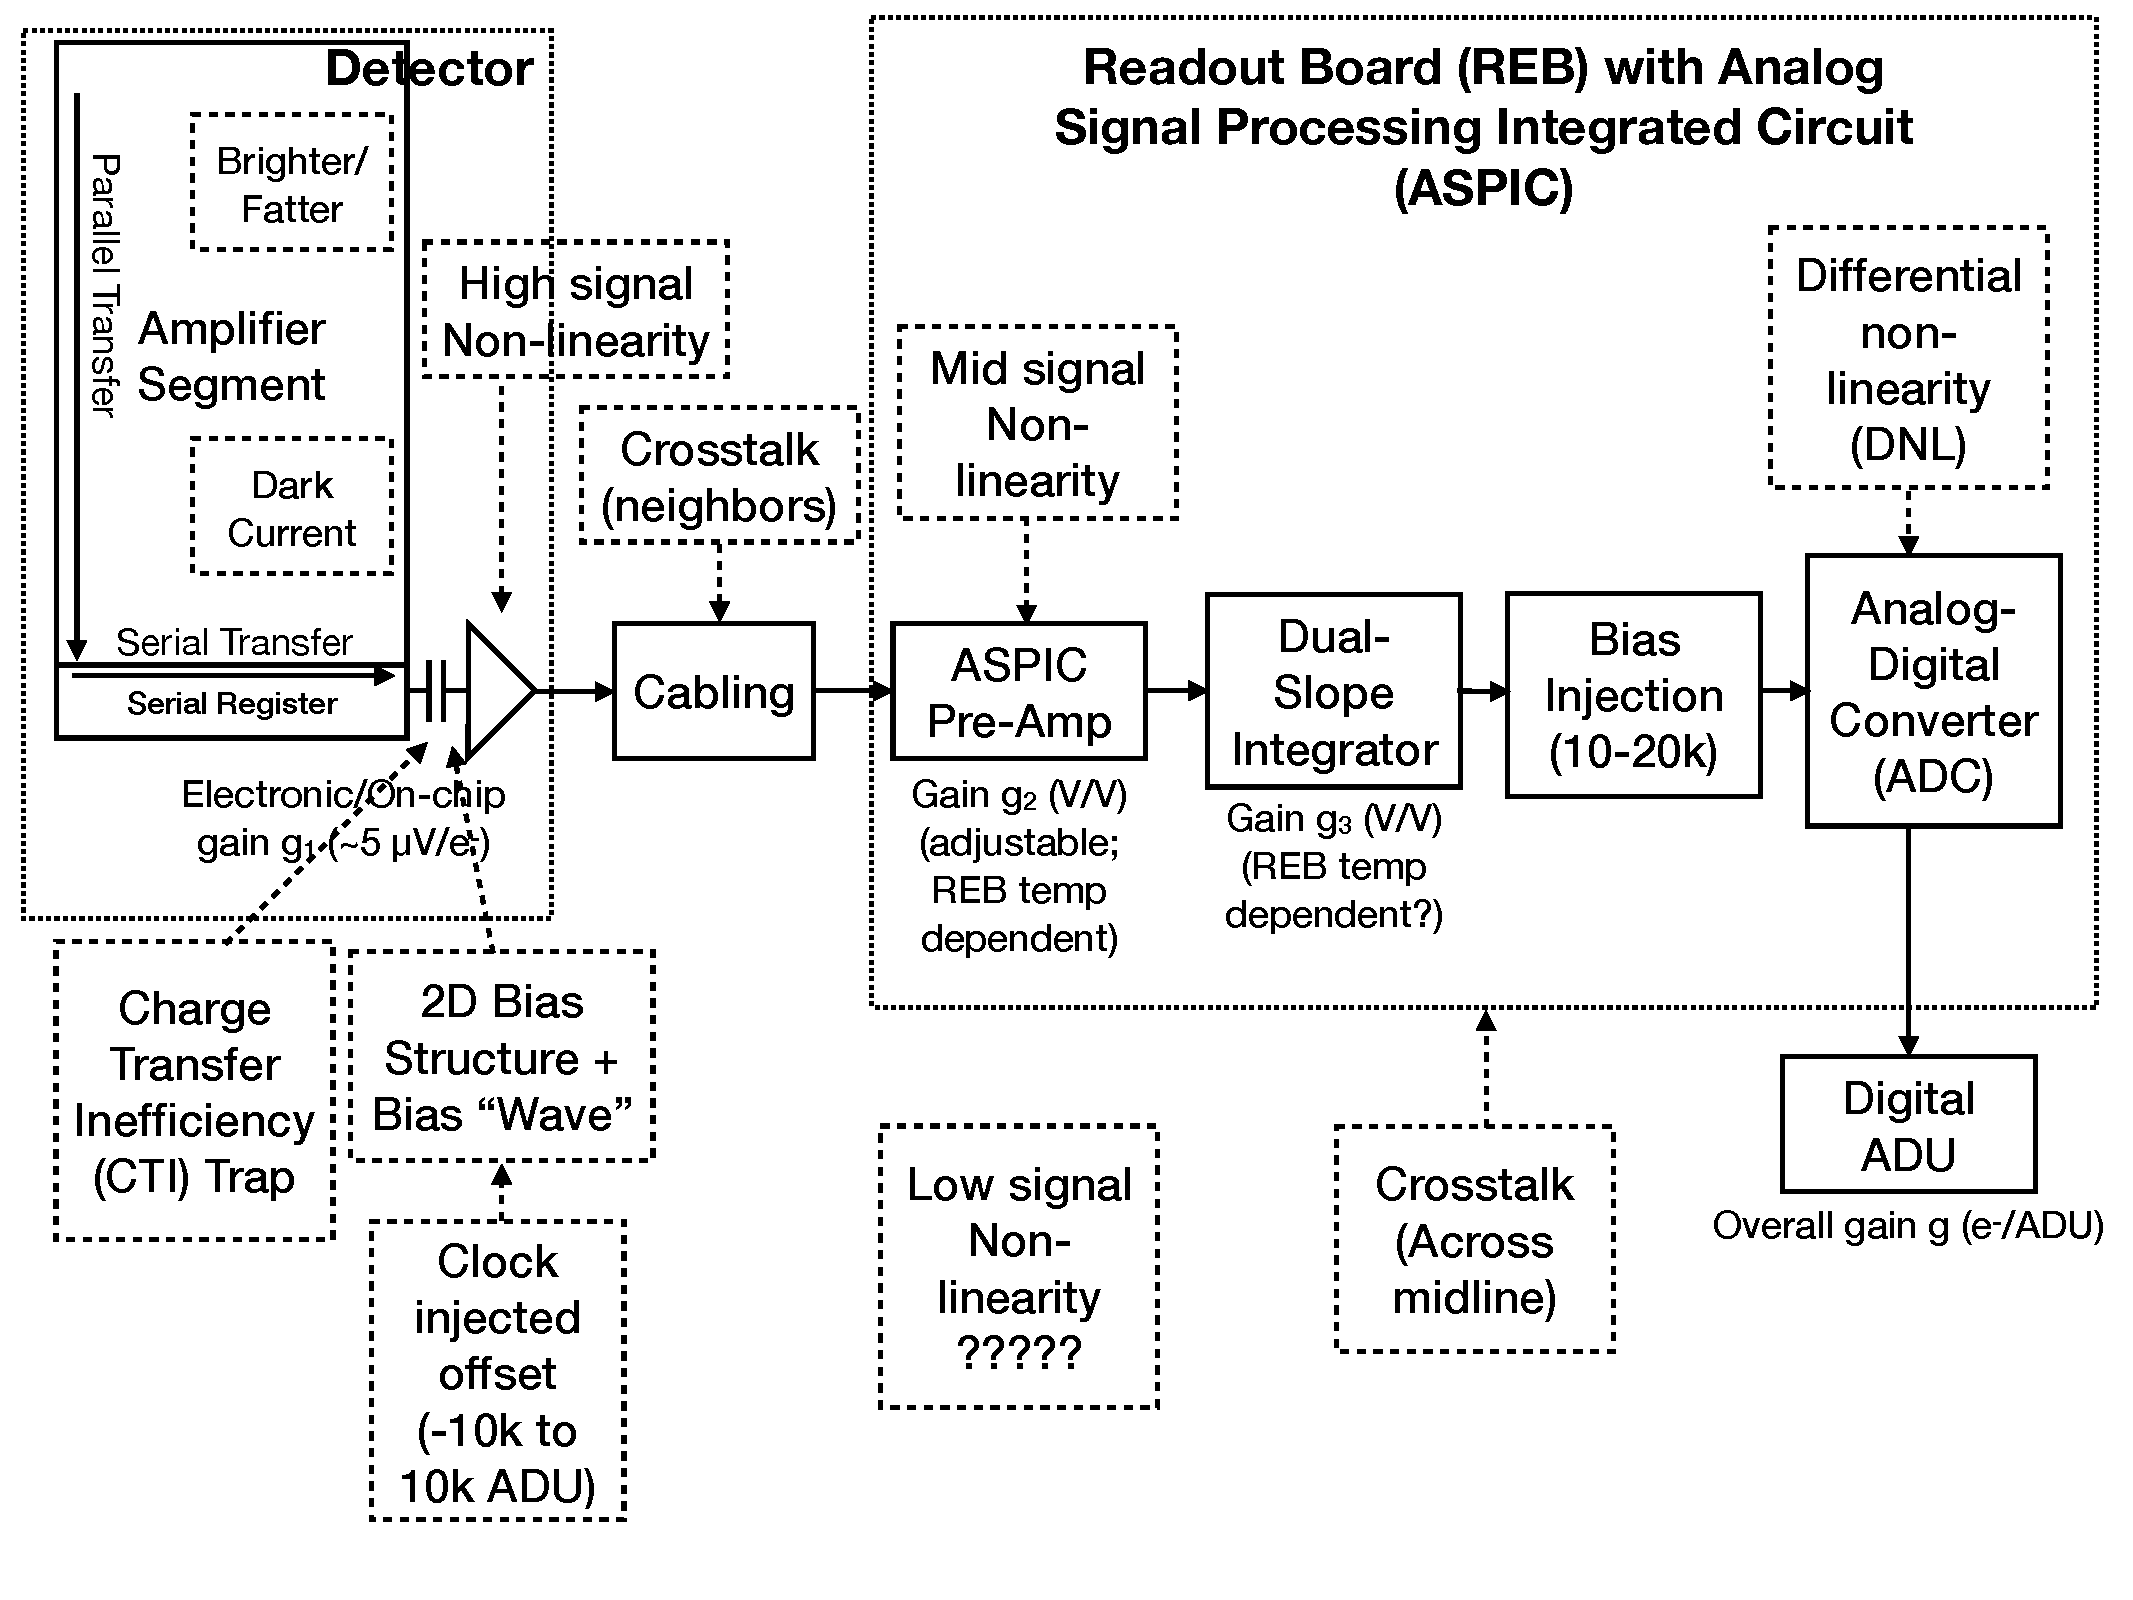
\includegraphics[width=\linewidth]{calibration_boxes_detector_model}
  \caption{The model of the detector and REB components, labeled with the effects that they impart on signal.}
  \label{fig:isr_signal_chain}
\end{figure}

\subsubsection{Background Subtraction}
\label{ssec:background_subtraction}

The background subtraction algorithms in the LSST Science Pipelines estimate and remove large-scale background signals from science imaging.
Such signals may include sky brightness from airglow, moonlight, scattered light instrumental effects, zodiacal light, and diffuse astrophysical emission.
In so doing, true astrophysical sources are isolated to allow for accurate detection and measurement.

To generate a \gls{background} model, each post-ISR image is divided into superpixels of $128\times128$ pixels.
Pixels with a mask flag set that indicates that they contain no useful science data or that they contain \gls{flux} from a preliminary source detection are masked.
The iterative $3\sigma$ clipped mean of the remaining pixels is calculated for each superpixel, constructing a \gls{background} statistics image.
A sixth-order Chebyshev polynomial is fit to these values on the scale of a single detector to allow for an extrapolation back to the native pixel resolution of the post-\gls{ISR} image.

\subsection{Calibration}
\label{ssec:drp_calibration}
Stars are detected in each post-\gls{ISR} image using a $5\sigma$ threshold.
Detections of the same star across multiple images are then associated to identify a consistent set of isolated stars with repeated observations suitable for use in PSF modeling, photometric \gls{calibration}, and astrometric \gls{calibration}.

Initial astrometric and photometric solutions are derived using only the calibration reference catalogs (see \secref{ssec:catalogs}), and an initial \gls{PSF} model is fit using PSFEx \citep{2011ASPC..442..435B}.
These preliminary solutions provide approximate source positions, fluxes, and \gls{PSF} shapes that serve as essential inputs to the \gls{calibration} process, enabling reliable source matching, selection of high-quality stars, and iterative refinement of the final astrometric, photometric, and \gls{PSF} models.
These preliminary solutions are subsequently replaced by more accurate fits, as described in the following sections.

\subsubsection{PSF Modeling}
\label{ssec:psf_modelling}
\gls{PSF} modeling in \gls{DP1} uses the Piff \citep{DES:2020vau} package.
Our configuration of Piff utilizes its \texttt{PixelGrid} model with a fourth-order polynomial interpolation per \gls{CCD}, except in the $u$-band, where star counts are insufficient to support a fourth-order fit.
In this case, a second-order polynomial is used instead.
Details on the choice of polynomial order, overall \gls{PSF} modeling performance, and known issues are discussed in \secref{ssec:psf_models}.

\subsubsection{Astrometric Calibration}
\label{ssec:global_astrometric_calibration}
Starting from the astrometric solution calculated in single frame processing (\secref{ssec:single_frame_processing}), the final astrometric solution is computed using the ensemble of visits in a given band that overlap a given \gls{tract}.
This allows the astrometric solution to be further refined by using all of the isolated point sources of sufficient signal-to-noise ratio in an image, rather than only those that appear in the reference catalog, as is done in single frame processing.
Using multiple whole visits rather than a single detector also allows us to account for effects that impact the full focal plane, and for the proper motion and parallax of the sources.

In order to perform the fit of the astrometric solution, isolated point sources are associated between overlapping visits and with the Gaia \gls{DR3} \citep{2023A&A...674A...1G} reference catalog where possible.
The model used for \gls{DP1} consists of a static map from pixel space to an intermediate frame (the per-detector model), followed by a per-visit map from the intermediate frame to the plane tangent to the telescope boresight (the per-visit model), then finally a deterministic mapping from the tangent plane to the sky.
The fit is done using the \texttt{gbdes} package \citep{2017PASP..129g4503B}, and a full description is given in \citet{DMTN-266}.

The per-detector model is intended to capture quasi-static characteristics of the telescope and camera. 
During \gls{Rubin Operations}, the astrometric solution will allow for separate epochs with different per-detector models, to account for changes in the camera due to warming and cooling and other discrete events.
However, for \gls{DP1}, \gls{LSSTComCam} was assumed to be stable enough that all visits use the same per-detector model. The model itself is a separate two-dimensional polynomial for each detector.
For \gls{DP1}, a degree 4 polynomial was used; the degree of the polynomial mapping is tuned for each instrument and may be different for LSSTCam.
Further improvements may be made by including a pixel-based astrometric offset mapping, which would be fit from the ensemble of astrometric residuals, but this is not included in the \gls{DP1} processing.

The per-visit model attempts to account for the path of a photon from both atmospheric sources and those dependent on the telescope orientation.
This model is also a polynomial mapping, in this case a degree 6 two-dimensional polynomial.
Correction for \gls{DCR} (\secref{sec:differential_chromatic_refraction}) was not done for \gls{DP1}, but will be included in LSSTCam processing during \gls{Rubin Operations}.
Future processing will also likely include a Gaussian Process fit to better account for atmospheric turbulence, as was demonstrated by \citet{2021AJ....162..106F} and \citet{2021A&A...650A..81L}.

The final component of the astrometric \gls{calibration} involves the positions of the isolated point sources included in the fit, which are described by five parameters: sky coordinates, proper motion, and parallax.
While proper motions and parallaxes are not released for DP1, they are fitted for these sources in the astrometric solution to improve the astrometric calibration.

\subsubsection{Photometric Calibration}
\label{photometric_calibration}
Photometric \gls{calibration} of the \gls{DP1} dataset is based on the \gls{FGCM} ~\citep[FGCM][]{2018AJ....155...41B}, adapted for the LSST Science Pipelines~\citep{2022PASJ...74..247A, SITCOMTN-086}.
We used the \gls{FGCM} to calibrate the full \gls{DP1} dataset with a forward model that uses a parameterized model of the atmosphere as a function of airmass along with a model of the instrument throughput as a function of wavelength.
The FGCM process typically begins with measurements of the instrumental throughput, including the mirrors, filters, and detectors.
However, because full scans of the \gls{LSSTComCam} as-built filters and individual detectors were not available, we instead used the nominal reference throughputs for the Simonyi Survey Telescope and LSSTCam.\footnote{Available at: \url{https://github.com/lsst/throughputs/tree/1.9}}
These nominal throughputs were sufficient for the \gls{DP1} calibration, given the small and homogeneous focal plane consisting of only nine \gls{ITL} detectors.
The FGCM atmosphere model, provided by MODTRAN~\citep{1999SPIE.3756..348B}, was used to generate a look-up table for atmospheric throughput as a function of zenith distance at Cerro Pachón.
This model accounts for absorption and scattering by molecular constituents of the atmosphere, including $O_2$ and $O_3$; absorption by water vapor; and Mie scattering by airborne aerosol particulates.
Nightly variations in the atmosphere are modeled by minimizing the variance in repeated observations of stars with a \gls{SNR} greater than 10, measured using ``compensated aperture fluxes''.
These fluxes include a local \gls{background} subtraction (see \secref{ssec:background_subtraction}) to mitigate the impact of \gls{background} offsets.
The model fitting process incorporates all six bands ($ugrizy$) but does not include any gray (achromatic) terms, except for a linear assumption of mirror reflectance degradation, which is minimal over the short duration of the \gls{DP1} observation campaign.
As an additional constraint on the fit, we use a subset of stars from the reference catalog~\citep{DMTN-277}, primarily to constrain the system's overall throughput and establish the ``absolute'' calibration.

\subsection{Visit Images and Source Catalogs}
\label{sssec:visit_images_source_catalogs}
With the final \gls{PSF} models, \gls{WCS} solutions, and photometric calibrations in place, we reprocess each single-epoch image to produce a final set of calibrated visit images and source catalogs.
Source detection is performed down to a $5\sigma$ threshold using the updated \gls{PSF} models, followed by measurement of \gls{PSF} and aperture fluxes.
These catalogs represent the best single-\gls{epoch} source characterization, but they are not intended for constructing light curves.
For time-domain analysis, we recommend using the \gls{forced photometry} tables described in \secref{sssec:lightcurves}.

\subsection{Coaddition Processing}
\label{ssec:coadd_processing}
\subsubsection{Coaddition}
\label{ssec:coaddition}
Only exposures with a \gls{seeing} better than 1.7 arcseconds FWHM are included in the deep coadded images. For the template coadds, typically only the top third of visits with the best \gls{seeing} are used (although see \secref{ssec:science_images} for more details), resulting in an even tighter image quality cutoff for the template coadds. Exposures with poor \gls{PSF} model quality, identified using internal diagnostics, are excluded to prevent contamination of the coadds with unreliable \gls{PSF} estimates. The remaining exposures are combined using an inverse-variance weighted mean stacking \gls{algorithm}.

To mitigate transient artifacts before coaddition, we apply the artifact rejection procedure described in \cite{DMTN-080} that identifies and masks features such as satellite trails, optical ghosts, and cosmic rays.
It operates on a time series of \gls{PSF}-matched images resampled onto a common pixel grid (``warps'') and leverages their temporal behavior to distinguish persistent astrophysical sources from transient artifacts.

Artifact rejection uses both direct (where no PSF-matching is performed) and PSF-matched warps, homogenized to a standard PSF of 1.8 arcseconds FWHM, broadly consistent with the 1.7 arcsecond FWHM \gls{seeing} threshold used in data screening.
A sigma-clipped mean of the \gls{PSF}-matched warps serves as a static sky model, against which individual warps are differenced to identify significant positive and negative residuals.
Candidate artifact regions are classified as \gls{transient} if they appear in less than a small percentage of the total number of exposures, with the threshold  based on the number of visits, $N$,  as follows:
\begin{itemize}
    \item $N=1$ or $2$: threshold $= 0$ (no clipping).
    \item $N=3$ or $4$: threshold $= 1$.
    \item $N=5$: threshold $= 2$.
    \item $N>5$: threshold $= 2+0.03N$.
\end{itemize}
Identified \gls{transient} regions are masked before coaddition, improving image quality and reducing contamination in derived catalogs.

\subsubsection{Detection, Deblending and Measurement}
\label{sssec:coadd_processing}
After constructing coadded images, sources are detected in each band, merged across bands, deblended, and measured to generate the final object catalogs  (\secref{ssec:catalogs}).
For each coadd in all six bands, we perform source detection at a $5\sigma$ detection threshold and then adjust the background with a per-patch constant (coadds are built from background-subtracted images, but the deeper detection on coadds redefines what is considered source versus background).
Detections across bands are merged in a fixed priority order, $irzygu$, to form a union detection catalog, which serves as input to deblending.

Deblending is performed using the Scarlet Lite algorithm, which implements the same model as Scarlet \citep{2018A&C....24..129M}, but operates on a single pixel grid.
This allows the use of analytic gradients, resulting in greater computational speed and memory efficiency.

\gls{Object} measurement is then performed on the deblended detection footprints in each band.
Measurements are conducted in three modes: independent per-band measurements, forced measurements in each band, and multiband measurements.

Most measurement algorithms operate through a single-band plugin system, largely as originally described in \citet{2018PASJ...70S...5B}.
The same plugins are run separately for each object on a deblended image, which uses the Scarlet model as a template to re-weight the original noisy coadded pixel values.
This effectively preserves the original image in regions where objects are not blended, while dampening the noise elsewhere.

A reference band is chosen for each object based on detection significance and measurement quality using the same priority order as detection merging ($irzygu$) and a second round of measurements is performed in forced mode using the shape and position from the reference band to ensure consistent colors \citep{2018PASJ...70S...5B}.

Measurement \gls{algorithm} outputs include object fluxes, centroids, and higher-order moments thereof like sizes and shapes. A variety of \gls{flux} measurements are provided, from aperture fluxes and forward modeling algorithms.

Composite model (CModel) magnitudes \citep{2004AJ....128..502A, 2018PASJ...70S...5B} are used to calculate the extendedness parameter, which functions as a star-galaxy classifier.
Extendedness is a binary classifier that is set to 1 if the PSF model flux is less than $98.5\%$ of the (free, not forced) CModel flux in a given band.
Additionally, the extendedness in the reference band is provided as a separate column for convenience as a multiband star-galaxy classification, and is recommended generally but also specifically for objects with low signal-to-noise ratio in some bands.

Gaussian-Aperture-and-PSF \citep[\gls{GAaP}][]{2008A&A...482.1053K, DMTN-190} fluxes are provided to ensure consistent galaxy colors across bands.
S\'ersic model \citep{1963BAAA....6...41S, 1968adga.book.....S} fits are run on all available bands simultaneously \cite[MultiProFit,][]{DMTN-312}.
The resulting S\'ersic model fluxes are provided as an alternative to CModel and are intended to represent total galaxy fluxes.
Like CModel, the S\'ersic model is a Gaussian mixture approximation to a true S\'ersic profile, convolved with a Gaussian mixture approximation to the \gls{PSF}.
CModel measurements use a double ``shapelet'' \citep{2003ARA&A..41..645R} PSF with a single shared shape, while the S\'ersic fits use a double Gaussian with independent shape parameters for each component.
S\'ersic model fits also include a free centroid, with all other structural parameters shared across all bands.
That is, the intrinsic model has no color gradients, but the convolved model may have color gradients if the \gls{PSF} parameters vary significantly between bands.

Further details on the performance of these algorithms are found in \secref{ssec:fluxes}.

\subsection{Variability Measurement}
\subsubsection{Difference Imaging Analysis}
\label{ssec:diffim_analysis}
Difference Image Analysis (DIA) uses the decorrelated Alard \& Lupton image differencing algorithm \citep{DMTN-021}.
We detected both positive and negative \texttt{DIASource}s at $5\sigma$ in the difference image.
Sources with footprints containing both positive and negative peaks due to offsets from the template position or blending were fit with a dipole centroid code, , which simultaneously fits offset positive and negative PSFs.

We filter a subset of \texttt{DIASource}s that have pixel flags characteristic of artifacts, non-astrophysical trail lengths, and unphysically negative direct fluxes.
We performed a simple spatial association of \texttt{DIASources} into \texttt{DIAObjects} with a one arcsecond matching radius.

The Machine Learning reliability model applied to DP1 was developed with the aim to meet the latency requirements for Rubin \gls{Alert Production} when executed on CPUs. Accordingly we developed a relatively simple model: a Convolutional Neural Network with three convolutional layers, and two fully connected layers.
The convolutional layers have a $5\times5$ kernel size, with 16, 32, and 64 filters, respectively.
A max-pooling layer of size 2 is applied at the end of each convolutional layer, followed by a dropout layer of 0.4 to reduce overfitting.
The last fully connected layers have sizes of 32 and 1.
The ReLU activation function is used for the convolutional layers and the first fully connected layer, while a sigmoid function is used for the output layer to provide a probabilistic interpretation.
The cutouts are generated by extracting postage stamps of $51\times51$ pixels centered on the detected sources.
The input data of the model consist of the template, science, and difference image stacked to have an array of \gls{shape} (3, 51, 51).
The model is implemented using PyTorch \citep{10.1145/3620665.3640366}.
The Binary Cross Entropy loss function was used, along with the \gls{Adam} optimizer with a fixed learning rate of $1\times10^{-4}$, weight decay of $3.6\times10^{-2}$, and a batch size of 128.
The final model uses the weights that achieved the best precision/purity for the test set.
Training was done on the \gls{S3DF} with an NVIDIA model L40S GPU.

The model was initially trained using simulated data from the second DESC Data Challenge (DC2; \citep{2021ApJS..253...31L}) plus randomly located injections of PSFs to increase the number of real sources, for a total of 89,066 real sources.
The same number of bogus sources were selected at random from non-injected DIASources.
Once the  \gls{LSSTComCam} data were available, the model was fine-tuned on a subset of the data containing 183,046 sources with PSF injections.
On the \gls{LSSTComCam} test set, the model achieved an accuracy of 98.06\%, purity of 97.87\%, and completeness of 98.27\%.
As discussed in \secref{sec:performance:dia}, the injections used to train this model version do not capture all types of astrophysical variability, so performance on the test set will not be representative for variable stars, comets, and other types of variable objects. 

\subsubsection{Light Curves}
\label{sssec:lightcurves}
To produce light curves, we perform multi-epoch \gls{forced photometry} on both the direct visit images and the difference images.
For light curves we recommend the \gls{forced photometry} on the difference images (\texttt{psDiffFlux} on the ForcedSource Table), as it isolates the variable component of the flux and avoids contamination from static sources.
In contrast, \gls{forced photometry} on direct images includes flux from nearby or blended static objects, and this contamination can vary with seeing.
Centroids used in the multi-epoch \gls{forced photometry} stage are taken either from object positions measured on the coadds or from the DIAObjects (the associated DIASources detected on difference images).

\subsubsection{Solar System Processing}
\label{sec:drp:solsys}

Solar system processing in \gls{DP1} consists of two key components: the association of observations (sources) with known solar system objects, and the discovery of previously unknown objects by linking sets of 
{\em tracklets}\footnote{A tracklet is defined as two or more detections of a moving object candidate taken in close succession in a single night.}.

To generate expected positions, ephemerides are computed for all objects found in the Minor Planet \gls{Center} orbit catalog using the \texttt{Sorcha} survey simulation toolkit (Merritt et al., in press)\footnote{Available at \url{https://github.com/dirac-institute/sorcha}}.
To enable fast lookup of objects potentially present in an observed visit, we use the {\tt mpsky} package \citep{mpsky}.
In each image, the closest DiaSource within 1~arcsecond of a known solar system object's predicted position is associated to that object.

Solar system discovery uses the {\tt heliolinx} package of asteroid identification and linking tools \citep{heliolinx}.
The suite consists of the following tasks:
\begin{itemize}
    \item Tracklet creation with {\tt make\_tracklets}
    \item Multi-night \gls{tracklet} linking with {\tt heliolinc}
    \item Linkage post processing (orbit fitting, outlier rejection, and de-duplication) with {\tt link\_purify}
\end{itemize}

The inputs to the \texttt{heliolinx} suite included all sources detected in difference images produced by an early processing of the \gls{LSSTComCam} commissioning data,  including some that were later rejected as part of \gls{DP1} processing and hence are not part of \gls{DP1}.

About 10\% of all commissioning visits targeted the near-ecliptic field Rubin\_SV\_38\_7 chosen to facilitate asteroid discovery.
Rubin\_SV\_38\_7 produced the vast majority of asteroid discoveries in DP1, as expected, but a few were found in off-ecliptic fields as well.

Tracklet creation with \texttt{make\_tracklets} used an upper limit angular velocity of 1.5 \gls{deg}/day, faster than any main belt asteroid and in the range of many \gls{NEO} discoveries.
To minimize false tracklets from fields observed multiple times per night, the minimum \gls{tracklet} length was set to three detections, and a minimum on-sky motion of five arcseconds was required for a valid \gls{tracklet}.

The heart of the discovery \gls{pipeline} is the \texttt{heliolinc} task, which connects (``links") tracklets belonging to the same object over a series of nights.
It employs the HelioLinC3D algorithm \citep{2020DPS....5221101E,2022DPS....5450404H}, a refinement of the original HelioLinC algorithm of \citet{2018AJ....156..135H}.

The \texttt{heliolinc} run tested each \gls{tracklet} with 324 different hypotheses spanning heliocentric distances from 1.5 to 9.8 \gls{au} and radial velocities spanning the full range of possible bound orbits (eccentricity 0.0 to nearly 1.0).
This range of distance encompasses all main belt asteroids and Jupiter Trojans, as well as many comets and Mars-crossers and some \glspl{NEO}.
Smaller heliocentric distances were not attempted here because nearby objects move rapidly across the sky and hence were not likely to remain long enough in an \gls{LSSTComCam} field to be discovered.
Candidate linkages, groups of tracklets whose propagated orbits cluster within a radius of 1.33 $\times\,10^{3}$ AU  at 1 AU, 
are identified, then post-processed via \texttt{link\_purify} to yeild a final, non‐overlapping set of high-confidence asteroid candidates, ranked by orbit-fit residuals and related metrics.
